\subsection{The Diffraction Grating}

A diffraction grating consist of a plate with \textbf{many closely spaced parallel slits} ruled on it.

When a parallel beam of monochromatic light is directed normally at a diffraction grating, light is \textbf{transmitted by the grating in certain directions only}
\begin{itemize}
    \item Light passing through each slit is diffracted.
    \item The diffracted light waves from adjacent slits \textbf{reinforce each other in certain directions only}, and \textbf{cancel out} in all other direction
\end{itemize}

The \textbf{central beam} - the zero order beam is in the same direction as the incident beam. Other transmitted beams are \textbf{numbered outwards} from the zero order beam.

The \textbf{angle of diffraction} increases if
\begin{itemize}
    \item Light of a \textbf{longer wavelength} is used.
    \item A grating of \textbf{closer slits} is used.
\end{itemize}

\subsubsection*{The Diffraction Grating Equation}
\begin{center}
    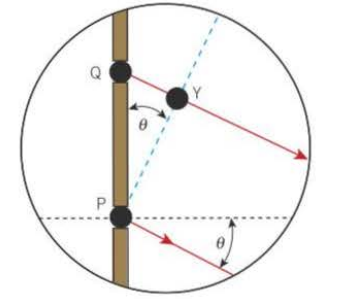
\includegraphics[width=4cm]{img/grating}
\end{center}

\begin{enumerate}
    \item For the formation of wavefront of the $n$th order beam, the wavefront emerging from slit $P$ \textbf{reinforces a wavefront emitted $n$ cycles earlier} by the adjacent slit $Q$
    \item The earlier wavefront therefore \textbf{travelled a distance} of $n$ wavelengths from the slit, so the distance $QY=n\lambda$
    \item Since the diffraction of the beam $\theta$ is \textbf{equal to the angle between the wavefront and the plane} of the slits. It follows that $$QY/QP$$
\end{enumerate}
Substituting variables gives the angle of diffraction for the $n$th order beam
$$d\sin\theta=n\lambda$$
where $d$ is the \textbf{grating spacing}, and the \textbf{number of slits per metre} on the grating $N=1/d$.

The \textbf{maximum number of orders} is given by the value $d/\lambda$ rounded down to the nearest whole number.

\subsubsection*{Types of Spectra}

\begin{itemize}
    \item \textbf{Continuous spectra} - spectrum of light from a filament lamp is a continuous spectrum of colour.
        \begin{itemize}
            \item The \textbf{most intense part} of the spectrum depends on the temperature of the light source.
            \item The \textbf{hotter the light source}, the shorter the wavelength of the brightest part of the spectrum.
            \item By measuring the wavelength of the brightest part of a continuous spectrum, we can therefore \textbf{measure the temperature} of the light source.
        \end{itemize}
    \item \textbf{Line emission spectra} - glowing gas in a \textbf{vapour lamp} or a \textbf{discharge tube} emits lights a \underline{specific wavelengths}, the spectrum consists of \textbf{narrow vertical lines} of different colours.
        \begin{itemize}
            \item The wavelengths of the lines are \textbf{characteristic of the chemical element} that produced the light.
            \item The \textbf{elements in a gas} can be identified by observing its line spectrum.
        \end{itemize}
    \item \textbf{Line absorption spectra} - continuous spectrum with \textbf{narrow dark lines} at certain wavelengths. E.g. the spectrum of light from a filament lamp observed after \textbf{passing through a glowing gas}.
        \begin{itemize}
            \item The pattern of dark lines is due to the elements in the glowing gas \textbf{absorbing light} of the same wavelength they can emit, but the emitted light is \textbf{not necessarily in the same direction} as the transmitted light.
            \item So the transmitted light is missing these wavelengths.
        \end{itemize}
\end{itemize}
